\documentclass[12pt]{article}

\baselineskip=20pt
\hsize=340pt
\vsize=490pt

\usepackage{amssymb}

\usepackage{color,graphicx}

\usepackage{amsmath}


\usepackage{amsmath,amssymb,amsthm}
\usepackage{pb-diagram}
%%%%%%%%%%%%%%%%%%%%%%%%%%%%%%%%%%%%%%%%%%%%%%%%%%%%%%%%%%%%%%%%%%%%%%%%%%%%%%%%%%%%%%%%%%%%%%%%%%% 
\usepackage{multicol}
\usepackage{color}
\usepackage{hyperref}
\usepackage{graphicx}
\usepackage[utf8x]{inputenc}
\usepackage[english,russian]{babel}

\newtheorem{Def}{Definition}[section]
\newtheorem{theorem}{Theorem}
\newtheorem{statement}{Statement}
\newtheorem{Cnj}[Def]{Conjecture}
\newtheorem{Prop}[Def]{Property}
\newtheorem{example}{Example}[section]


\newcommand{\go}{\stackrel{\circ }{\mathfrak{g}}}
\newcommand{\ao}{\stackrel{\circ }{\mathfrak{a}}}
\newcommand{\co}[1]{\stackrel{\circ }{#1}}
\newcommand{\pia}{\pi_{\mathfrak{a}}}
\newcommand{\piab}{\pi_{\mathfrak{a}_{\bot}}}
\newcommand{\gf}{\mathfrak{g}}
\newcommand{\gfh}{\hat{\mathfrak{g}}}
\newcommand{\af}{\mathfrak{a}}
\newcommand{\afh}{\hat{\mathfrak{a}}}
\newcommand{\bff}{\mathfrak{b}}
\newcommand{\afb}{\mathfrak{a}_{\bot}}
\newcommand{\hf}{\mathfrak{h}}
\newcommand{\hfg}{\hf_{\gf}}
\newcommand{\hfa}{\hf_{\af}}
\newcommand{\hfb}{\mathfrak{h}_{\bot}}
\newcommand{\pf}{\mathfrak{p}}
\newcommand{\aft}{\widetilde{\mathfrak{a}}}
\newcommand{\sfr}{\mathfrak{s}}


\begin{document}

\title{Сплинты корневых систем для специальных подалгебр Ли}

\author{В.Д.~Ляховский$^1$, А.А.~Назаров$^{1,2}$, П.И.~Какинь$^{1}$\\
  {\small $^1$ Кафедра физики высоких энергий и элементарных частиц,}\\ {\small Санкт-Петербургский государственный университет}\\
  {\small 198904, Санкт-Петербург, Россия}\\
  {\small $^{2}$ e-mail: antonnaz@gmail.com}}
%\date{}
%\address{ $^1$ Department of High-energy and elementary particle physics,  St Petersburg State University, 198904, Saint-Petersburg, Russia}
%\address{ $^{2}$ e-mail: anton.nazarov@hep.phys.spbu.ru}

\maketitle

\begin{abstract}
  Расщепление или сплинт -- это разложение корневой системы в объединение нескольких корневых
  систем. Сплинт возникает при изучении (регулярных) вложений редуктивных подалгебр. Его можно
  использовать для построения правил ветвления представлений. Мы рассматриваем специальное вложения
  подалгебры Ли в простые алгебры Ли, классифицируем проекции корневых систем алгебр и выводим
  условия возникновения сплинта и совпадения коэффициентов ветвления с кратностями весов. Хотя
  такое совпадение происходит не слишком часто, оно оказывается связано с базисом Гельфанда-Цетлина. 

\noindent{\it Keywords\/}: Алгебра Ли, специальная подалгебра, ветвление, кратность весов, сплинт
\end{abstract}


\section{Введение}
\label{sec:introduction}

Понятие сплинта (расщепления) было предложено Дэвидом Рихтером в работе \cite{richter2008splints}.
Сплинт -- это разложение корневой системы в объединение образов двух или более вложений других
корневых систем. Вложением  $\phi$ корневой системы $\Delta_1$ в корневую систему  system $\Delta$
называется биективное отображение корней $\Delta_{1}$ в (собственное) подмножество  $\Delta$,
коммутирующее с  законом сложения векторов в $\Delta_{1}$ и $\Delta$.
\begin{equation*}
\phi:\Delta_1 \longrightarrow \Delta
\end{equation*}
\begin{equation*}
\phi \circ (\alpha + \beta) =\phi \circ \alpha + \phi \circ \beta,
\,\,\, \alpha,\beta \in \Delta_1
\end{equation*}

Заметим, что мы не требуем от образа $Im(\phi)$ сохранения свойств корневой системы за исключением
совпадения правил сложения с правилами сложения в $\Delta_{1}$ (для прообразов). Если вложение
$\phi$ сохраняет углы между корнями, то оно называется ``метрическим''. Два вложения $\phi_1$ и
$\phi_2$ расщепляют корневую систему $\Delta$, если последняя может быть представлена в виде
дизъюнктного образов $Im(\phi_1)$ и $Im(\phi_2)$.

Чем же интересны отображения корневых систем, не сохраняющие углов между корнями? Аддитивные
свойства корневой системы определяют структуру модуля Верма:
    \begin{equation*}
      M^{\mu}=U(\gf)\underset{U(\bff_{+})}{\otimes} D^{\mu}(\bff_{+})=\{(E^{-\alpha_{1}})^{n_{1}}\dots (E^{-\alpha_{s}})^{n_{s}} \left|v_{\mu}\right>\}_{\alpha_{i}\in\Delta^{+}}^{n_{i}=0,1,\dots}
    \end{equation*}
Здесь $\bff_{+}$ -- подалгебра Бореля алгебры $\gf$, $D^{\mu}$ -- одномерное представление
подалгебры Бореля, $\left|v_{\mu}\right>$ -- вектор старшего веса, а  $E^{-\alpha_{j}}$ --
понижающие операторы, соответствующие положительным корням $\alpha_{j}\in \Delta^{+}$. 
Формула Вейля для характеров выражает характер неприводимого представления в виде комбинации характеров
модулей Верма: 
\begin{equation*}
  \mathrm{ch} L^{\mu}=\frac{\sum_{w\in W} \varepsilon(w) e^{w(\mu+\rho)-\rho}}{\sum_{w\in W}\varepsilon(w) e^{w\rho-\rho}}=\sum_{w\in W} \varepsilon(w)\; \mathrm{ch} M^{w(\mu+\rho)-\rho}
\end{equation*}
Здесь суммирование ведется по элементам группы Вейля, действие которых $w\triangleright \mu
=w(\mu+\rho)-\rho$ зависит от углов между корнями. Но формулу Вейля для характеров можно переписать,
представив элементы группы Вейля в виде произведений отражений $s_{\alpha}, \alpha \in S$ в
гиперплоскостях, ортогональных простым корням: $w=s_{\alpha_{1}}\cdot s_{\alpha_{2}}\dots$.
Отражения действуют на корневую систему перестановками, так что композицию такого действия с
вложением $\phi$ нетрудно вычислить. Орбиту группы Вейля $w\triangleright \mu, w\in W$ можно
построить последовательными вычитаниями корней из старшего веса $\mu$. Для этого обозначим индексы
Дынкина веса $\mu$ через $(\mu_{1},\dots \mu_{r})$. Тогда $\mu-\mu_{1}\alpha_{1},
\mu-\mu_{2}\alpha_{2},\dots, \mu-\mu_{r}\alpha_{r}, \alpha_{i}\in S$ -- это веса орбиты, которые
получаются из старшего веса $\mu$ элементарными отражениями $s_{\alpha_{i}}, \alpha_{i}\in S$.
Следующий набор точек орбиты, получаемых последовательным применением двух отражений
$s_{\alpha_{i}}\cdot s_{\alpha_{j}}\triangleright\mu$, можно построить путем вычитания
$\mu-\mu_{i}\alpha_{i}-\mu_{j} (s_{\alpha_{i}}\alpha_{j})$. Продолжая данную процедуру, мы построим
образ сингулярного элемента $\Psi=\sum_{w\in W} \varepsilon(w) e^{w(\mu+\rho)-\rho}$ под действием
вложения $\phi$ \cite{2011arXiv1111.6787L}. Кратности в характере модуля Верма не меняются при
вложении, так как они определяются аддитивными свойствами корней. Соответственно, при вложении
сохраняются и кратности в неприводимых модулях.

Корневая система регулярной подалгебры содержится в корневой системе алгебры, так что сплинт
возникает при вычислении коэффициентов ветвления. 

В работе  \cite{2011arXiv1111.6787L} было показано, что существование сплинта ведет к совпадению
коэффициентов ветвления с кратностями весов при выполнении некоторых дополнительных условий.
Обозначим алгебру Ли через $\gf$ и рассмотрим ее подалгебру $\af$. Если подалгебра  $\af$ регулярна,
то ее корневая система  $\Delta_{\af}$ содержится в $\Delta_{\gf}$. Коэффициенты ветвления $b^{(\mu)}_{\nu}$
появляются при разложении неприводимого представления  $L^{\mu}_{\gf}$ алгебры $\gf$ в сумму
неприводимых представлений подалгебры $\af$:
\begin{equation}
  \label{eq:1}
  L^{\mu}_{\gf}=\bigoplus_{\nu} b^{(\mu)}_{\nu} L^{\nu}_{\af}
\end{equation}

Предположим, что корневая система $\Delta_{\gf}$ расщепляется как  $\Delta_{\gf}=\Delta_{\af} \cup
\phi(\Delta_{\sfr})$, где  $\phi$ -- вложение корневой системы $\Delta_{\sfr}$ некоторой полупростой
алгебры Ли $\sfr$. Тогда коэффициенты ветвления $b^{(\mu)}_{\nu}$ при редукции
$L^{(\mu)}_{\gf\downarrow \af}$ совпадают с кратностями весов  $m^{(\tilde \mu)}_{\nu}$ в
представлениях  $\sfr$ при выполнении определенного технического условия \cite{2011arXiv1111.6787L}.
Старший вес  $\tilde\mu$ представления $\sfr$ вычисляется по индексам Дынкина старшего веса  $\mu$
модуля алгебры $\gf$. Доказательство равенства коэффициентов ветвления с кратностями весов
представлений $\sfr$ основывается на разложении сингулярного элемента алгебры  $\gf$ в комбинацию
сингулярных элементов $\sfr$:
\begin{equation}
 \Phi ^{\mu }_{\gf} = \sum_{w\in W_{\frak{a}}}\epsilon\left( w\right)w\left( e^{\mu +\rho _{\gf}}\phi\left( e^{-\widetilde{\mu }}\Psi^{\widetilde{\mu }}_{\sfr}\right)\right),
\end{equation}
где $\epsilon\left( w\right)$ -- определитель элемента $w$ группы Вейля $W_{\af}$ подалгебры $\af$.
Действие группы Вейля на весах продолжается на алгебры формальных экспонент по правилу
$w\left(e^{\nu}\right)=e^{w\nu}, w\in W$. Отсюда кратность $M_{\left( \sfr\right) \widetilde{\nu
  }}^{\widetilde{\mu }}$ веса $\widetilde{\nu }$ из весовой диаграммы представления алгебры $\sfr$
со старшим весом $\tilde\mu$ определят коэффициент ветвления $b_{\nu }^{(\mu )}$ для старшего веса
$\nu =\left( \mu -\phi \left( \widetilde{\mu }-\widetilde{\nu }\right) \right) $:
\begin{equation}
b_{\left( \mu -\phi \left( \widetilde{\mu }-\widetilde{\nu }\right) \right)
}^{(\mu )}=M_{\left( \sfr\right) \widetilde{\nu }}^{\widetilde{\mu }}. 
\label{bran1}
\end{equation}

В данной работе мы воспользуемся похожим подходом для изучения специальных вложений. Мы
рассматриваем специальные вложения подалгебр Ли в алгебру Ли. В таком случае корневая система
подалгебры на содержится в корневой системе алгебры и первоначальная мотивация для введения сплинта
не применима. Но мы можем рассмотреть проекцию корневой системы алгебры на корневое пространство
подалгебры. Результат такой проекции уже не будет корневой системой, однако он будет удовлетворять
более мягким условиям (см Раздел \ref{sec:spec-embedd-proj}). Оказывается, что сплинты проекций
корневых систем можно классифицировать, используя разложение присоединенного представления алгебры
в прямую сумму представлений подалгебры. Мы показываем, что при наличии такого сплинта коэффициенты
ветвления совпадают с кратностями весов в представлениях другой алгебры Ли (Раздел
\ref{sec:splints-spec-embedd}). А значит, в этом случае коэффициенты ветвления очень легко вычислить.

Мы используем теорию представлений подалгебры для классификации всех сплинтов для проекции корневой
системы алгебры. Однако метод универсален и мы применяем его и к метрическим сплинтам и регулярным
подалгебрам. В результате мы получаем правила Гельфанда-Цетлина для регулярных и специальных
вложений. 

В заключении \ref{sec:conclusion} мы обсуждаем случаи, которые не укладываются в упомянутую выше
классификацию.


\section{Специальные вложения и проекции корневой системы}
\label{sec:spec-embedd-proj}

Специальные вложения подалгебр детально рассматривались в фундаментальных работах Евгения
Борисовича Дынкина \cite{dynkin1952semisimple,dynkin1952maximal}, где для них использовалось
название ``S-подалгебры'' чтобы отличить от регулярных или ``R-подалгебр'', полученных путем
исключения некоторых корней из корневой системы алгебры. Все регулярные подалгебры нетрудно построить
путем исключения вершин из расширенной диаграммы Дынкина для алгебры, но для специальных подалгебр
такого простого метода нет. Полная классификация для исключительных алгебр Ли была построена недавно
в работе \cite{minchenko2006semisimple}. Алгоритм построения специальных подалгебр реализован в виде
пакета для системы GAP, но построение все равно требует участия человека \cite{de2011constructing}.  

Будем предполагать, что алгебра Ли $\gf$ простая. Обозначим подалгебру через $\af$. Соответствующие
подалгебры Картана будем обозначать через $\hfg$ и $\hfa$, и отождествим их с дуальными
пространствами $\hfg^{*}$, $\hfa^{*}$ используя формы Киллинга алгебр  $\gf$ и $\af$.

Для построения вложения  $\af\to\gf$ надо отождествить некоторое представление  $L^{\nu}_{\af}$ с
подпространством в алгебре Ли $\gf$. Затем необходимо проверить, что генераторы  $\af$ могут быть
представлены в виде линейных комбинаций генераторов  $\gf$. После отождествления подалгебры Картана
$\hfa\subset \af$ с дуальным пространством $\hfa^{*}$ при помощи формы Киллинга, корневую систему
$\Delta_{\gf}$ алгебры $\gf$ можно спроектировать на  $\hfa^{*}$ используя выражение
генераторов подалгебры $\hfa$ через генераторы  $\hfg$.

%%  To reduce $\gf$-representations project $\gf$ root system to Cartan subalgebra of $\af$. 
%% 
%%  To construct an embedding of special subalgebra $\af\to \gf$ one
%% needs to consider some representation of $\af$ of dimension $\mathrm{dim}\gf$ and
%% identify generators of $\af$ with linear combinations of generators of $\gf$ in
%% the adjoint representation. 
%% 
%%  Such subalgebras are constructed by considering
%% representation of the algebra to
%% 

Свойства этой проекции описаны в классических работах  \cite{dynkin1952semisimple,dynkin1952maximal} в
следующих теоремах:

\begin{theorem}\label{dyn0}
  Если представление  $L^{\mu}_{\gf}$ алгебры $\gf$ индуцирует представление $L^{\tilde\mu}_{\af}$
  подалегбры $\af$, то весовая диаграмма $L^{\tilde\mu}_{\af}$ получается из диаграммы
  $L^{\mu}_{\gf}$ ортогональной проекцией $\hfg^{*}$ на $\hfa^{*}$.
  \cite{dynkin1952maximal}. 
\end{theorem} 

Применяя эту теорему к присоединенному представлению  $\gf$, видим, что проекция корневой
системы  $\Delta_{\gf}$ на $\hfa^{*}$ оказывается весовой системой некоторого конечномерного но не
обязательно неприводимого представления $\af$. Более того, это приводимое представление должно
содержать присоединенное представление $\af$. Если обозначить проекцию корневой системы через
\begin{equation}
  \label{eq:2}
  \Delta'=\pia\left(\Delta_{\gf}\right),
\end{equation}
то все корни $\af$ будут содержаться в $\Delta'$. То есть система  $\Delta'$ может быть корневой
системой, но она не обязательно является приведенной и может содержать некоторые векторы с
кратностью больше единицы.

Следующие теоремы \cite{dynkin1952semisimple} также описывают свойства  $\Delta'$. 

\begin{theorem}\label{dyn1}
  Каждая специальная подалгебра  $\af$ полупростой алгебры Ли  $\gf$ -- целочисленная, то есть
  проекции корней  $\gf$ на $\hfa^{*}$ являются линейными комбинациями простых корней  $\af$ с
  целочисленными коэффициентами \cite{dynkin1952semisimple}
\end{theorem}

\begin{theorem}\label{dyn2}
  Если $\af$  -- полупростая подалгебра полупростой алгебры Ли $\gf$ и генератор $e_{\alpha}$,
  соответствующий корню $\alpha$ алгебры $\af$, представляется в виде линейной комбинации  $e_{\alpha}=\sum_{\beta}
  e_{\beta}$ генераторов $\gf$ соответствующих корням  $\beta$ алгебры $\gf$, тогда все эти корни
  $\beta$ проектируются в  $\alpha$,
  $\pia(\beta)=\alpha$. 
  \cite{dynkin1972semisimple,dynkin1952semisimple}. 
\end{theorem}

Из этих теорем мы видим, что  корневая система $\Delta_{\af}$ вложена метрически (в смысле
определения сплинта) в проекцию  $\Delta'$. Более того, кратности некоторых корней 
$\alpha\in\Delta_{\af}$ в этой проекции  $\Delta'$ больше единицы. 

Например, проекция корневой системы $D_{4}$($so(8)$) на корневую систему специальной подалгебры
$A_{2}$($su(3)$) совпадает с корневой системой $G_{2}$, но кратность коротких корней равна $3$.


%% Relying on these theorems we can encode the projections of root system by Dynkin diagrams. We need
%% to allow simple roots to have non-trivial multiplicities. 
%% 

\section{Сплинты для специальных вложений}
\label{sec:splints-spec-embedd}

%Since roots are weights of the adjoint representation, such a projection produces the weight diagram
%of $\af$-representation that contains adjoint representation of $\af$.
%After the subtraction of
%$\af$-root system $\Delta_{\af}$ from $\Delta'$ we obtain the weight diagram of representation called
%``characteristic representation of subalgebra $\af$'' by Dynkin in the seminal paper
%\cite{dynkin1952semisimple}.

Мы хотим перечислить все случаи совпадения коэффициентов ветвления с кратностями весов в
представлении некоторой другой алгебры. Такое совпадение возможно, если проекция $\Delta'$ корневой
системы алгебры $\gf$ допускает сплинт $\Delta'=\varphi_{\af}(\Delta_{\af})\cup
\varphi_{\sfr}(\Delta_{\sfr})$, где  $\varphi_{\af}$ и $\varphi_{\sfr}$ -- вложения соответствующих
корневых систем. Вложение  $\varphi_{\af}$ метрическое и тривиальное. Кроме этого, проекция
сингулярного элемента  $\pia\left(\Psi^{\mu}_{\gf}\right)$ должна раскладываться в линейную
комбинацию сингулярных элементов неприводимых представлений $\sfr$:
\begin{equation}
  \label{eq:4}
  \pia\left(\Psi^{\mu}_{\gf}\right)=\sum_{\nu} \varkappa_{\nu}e^{\nu}\Psi^{\tilde\mu}_{\sfr},
\end{equation}
с целыми коэффициентами  $\varkappa_{\nu}$, где  множество весов  $\nu$, по которому ведется
суммирование, будет определено ниже. Это разложение сингулярного элемента очень похоже на ветвления
орбит группы Вейля, рассмотренные в работах  \cite{larouche2011branching,larouche2009branching}.
Сперва мы перечислим все расщепления проекций корневой системы в объединение простых корневых систем
при специальных вложениях, а затем обсудим разложение сингулярного элемента. 

Проекция  $\Delta'$ корневой системы  $\gf$ совпадает с проекцией весовой диаграммы присоединенного
представления алгебры  $\gf$, за исключением нулевого веса. Присоединенное представление  $\gf$
содержит присоединенное представление  $\af$ и раскладывается в прямую сумму
\begin{equation}
  \label{eq:3}
  \mathrm{ad}_{\gf}=\mathrm{ad}_{\af}\oplus M_{\af}^{\chi},
\end{equation}
где  $M^{\chi}_{\af}$ -- не обязательно неприводимое представление $\af$, названное 
``характеристическим'' в работе \cite{dynkin1952semisimple}. 


Весовая диаграмма $M^{\chi}_{\af}$ совпадает с корневой системой  $\Delta_{\sfr}$, за исключением
нулевого веса. То есть нам достаточно найти все представления для всех простых алгебр Ли $\af$
такие, что их весовая диаграмма совпадает с некоторой корневой системой после исключения нулевого
веса. Во-первых, заметим, что все веса  $M^{\chi}_{\af}$ должны быть  не меньшей длины чем
кратчайший корень $\af$, так как $\af$ -- целочисленная подалгебра $\gf$ \ref{dyn1}. Во-вторых,
$M^{\chi}_{\af}$ должна содержать веса не более, чем двух разных длин. 

Если в корневой системе  $\Delta_{\gf}$ есть корни $\alpha: \alpha\perp \beta,\; \forall \beta\in
\Delta_{\af},$ ортогональные корневой системе подалгебры, то сингулярный элемент не допускает
разложения \ref{eq:4}.  В этом случае элементы формальной алгебры $e^{\nu}$ проекции
$\pia\left(\Psi^{\mu}_{\gf}\right)$ надо снабдить размерностями представлений алгебры $\afb$,
порожденной генераторами, соответствующими ортогональным корням \cite{2010arXiv1007.0318L}. Тогда
правая часть разложения  \ref{eq:4} будет содержать нетривиальные кратности и совпадение
коэффициентов ветвления с кратностями весов в представлениях  $\sfr$ не будет иметь места. В
этом случае можно вывести более сложное соотношение между кратностями весов и коэффициентами
ветвления, но этот вывод лежит за рамками данной работы. 

Кратность нулевого веса в присоединенном представлении равна рангу алгебры. Так что при 
$\mathrm{rank}\gf-\mathrm{rank}\af=1$, характеристическое представление  $M^{\chi}_{\af}$ должно
быть свободно от нетривиальных кратностей.  При $\mathrm{rank}\gf-\mathrm{rank}\af>1$ только нулевой
вес может иметь нетривиальную кратность. 

Простейшие свободные от кратностей представления называется ``строго свободными от кратностей''
 (``strongly multiplicity free'') \cite{lehrer2006strongly} и представляют собой представления с
 весовыми системами, допускающими строгое упорядочение $\nu_{1}<\nu_{2} \Leftrightarrow
 \nu_{1}=\nu_{2}+n \alpha$, где $n\in
\mathbb{N}, \alpha\in \Delta^{+}_{\af}$ и для всех $\nu_{1},\nu_{2}$ либо $\nu_{1}<\nu_{2}$, либо
$\nu_{2}<\nu_{1}$.

Список строго свободных от кратностей представлений состоит из (первых) фундаментальных
представлений в сериях $A_{r}, B_{r}, C_{r}$, представления исключительной алгебры Ли $G_{2}$
(7-мерного) и всех представлений $A_{1}$. 

Фундаментальные веса алгебры $A_{r}$ короче, чем ее корни, но проекции весов $\gf$ должны даваться
линейными комбинациями корней специальной подалгебры  $\af$ с целыми коэффициентами, так что первый
класс строго свободных от кратностей представлений не порождает проекции корневой системы,
допускающей расщепление.

Тем не менее, объединение диаграмм двух фундаментальных представлений  $A_{2}$ с корневой системой
$A_{2}$ образует корневую систему $G_{2}$. Этот случай соответствуют сплинту
$\Delta_{G_{2}}=\varphi_{1}( \Delta_{A_{2}})\cup \varphi_{2}(\Delta_{A_{2}})$, связанному с
регулярной подалгеброй $A_{2}\subset G_{2}$ (подробнее см. \cite{2011arXiv1111.6787L}).

Первое фундаментальное представление  $B_{r}$ немедленно дает сплинт $\Delta'=\pi_{B_{r}}\left(
\Delta_{D_{r+1}}\right) = \Delta_{B_{r}}\cup \Delta_{A_{1}+\dots+A_{1}}$, соответствующий правилу
ветвления Гельфанда-Цетлина с тривиальными коэффициентами для специального вложения
$\mathfrak{so}(2r+1)\to \mathfrak{so}(2r+2)$.

Длина первого фундаментального веса алгебры   $C_{r}$ меньше, чем длина ее короткого корня, так что
этот случай не может порождать сплинт для целочисленной подалгебры. 

Далее, если в проекции  $\Delta'$ на подалгебру  $A_{1}$ есть векторы разной длины, то в такой
проекции есть нетривиальные кратности и система $\Delta_{\sfr}$ должна содержать сонаправленные
корни. Простейший пример -- это специальное вложение $A_{1}\to A_{2}$ с индексом 4, где
$\Delta_{\sfr}$ -- это корневая система $BC_{1}$. Такие системы не соответствуют полупростым
алгебрам Ли, так что мы не можем говорить о совпадении коэффициентов ветвления для редукции
$\gf\downarrow \af$ с кратностями весов в представлениях $\sfr$.

%% The only case of the projection $\Delta'$ to $A_{1}$ with root multiplicities not greater than 2 is
%% special embedding $A_{1}\to A_{2}$ with index 1 given by 
%% 

Наконец, весовая диаграмма семимерного представления $G_{2}$ вместе с корневой системой $G_{2}$
образует проекцию корневой системы $B_{3}$, возникающую при специальном вложении $G_{2}\to B_{3}$.
Коэффициенты ветвления в этом случае совпадают с кратностями весов в представлениях алгебры $G_{2}$.

Полная классификация представлений, свободных от кратностей, получена в работе
\cite{howe1995perspectives} (см. также \cite{stembridge2003multiplicity}). Она состоит из
микровесовых и квазимикровесовых представлений.

Вес  $\mu$ называется микровесом, если  $\left<\mu,\alpha^{\vee}\right>\leq 1$ для всех $\alpha\in
\Delta^{+}$ и все веса неприводимого представления  $L^{\mu}$ лежат на той же орбите группы Вейля,
что и $\mu$. Вес называется квазимикровесом, если $\left<\mu,\alpha^{\vee}\right>\leq 2$ для всех
$\alpha\in \Delta^{+}$ и все ненулевые веса представления лежат на одной орбите группы Вейля.

Микровесовые представления хорошо изучены и очень полезны при вычислениях, например, тензорных произведений
\cite{stembridge2003multiplicity,stembridge2001computational}. Микровесовые представления нумеруются
элементами весовой решетки, факторизованной по корневой решетке. Для каждой простой алгебры Ли
существует единственное квазимикровесовое представление, не являющееся микровесовым.  Кратность
нулевого веса в квазимикровесовом представлении равна числу коротких вершин в диаграмме Дынкина.

Полный список микровесовых представлений состоит из тензорных степеней векторного представления
алгебр серии $A_{r}$; спинорных представлений алгебр серии $B_{r}$; векторных представлений $C_{r}$;
векторных и полуспиновых представлений $D_{r}$; двух 
27-мерных представлений алгебры $E_{6}$ и  56-мерного представления $E_{7}$. 

Квазимикровесовые представления, не являющиеся микровесовыми -- это присоединенное представление
$A_{r}$, векторное представление $B_{r}$, представление размерности $2r^{2}-r-1$ алгебры $C_{r}$,
присоединенные представления алгебр $D_{r}, E_{6}, E_{7}, E_{8}$, 26-мерное представление $F_{4}$ и
7-мерное представление $G_{2}$.

%% 
%%     An (n+1
%%     k) for 0 ≤ k ≤ n (exterior powers of vector representation). Quasi-minuscule: n2+2n (adjoint)
%%     Bn 1 (trivial), 2n (spin). Quasi-minuscule: 2n+1 (vector)
%%     Cn 1 (trivial), 2n (vector). Quasi-minuscule: 2n2–n–1 if n>1
%%     Dn 1 (trivial), 2n (vector), 2n−1 (half spin), 2n−1 (half spin). Quasi-minuscule: 2n2–n (adjoint)
%%     E6 1 , 27, 27. Quasi-minuscule: 78 (adjoint)
%%     E7 1, 56. Quasi-minuscule: 133 (adjoint)
%%     E8 1. Quasi-minuscule: 248 (adjoint)
%%     F4 1. Quasi-minuscule: 26
%%     G2 1. Quasi-minuscule: 7
%% 
%% 

Классификация неприводимых представлений  $L^{\mu}$, свободных от кратностей, в работе
\cite{howe1995perspectives,stembridge2003multiplicity} состоит из следующих классов:
\begin{itemize}
\item (1) $\mu$ -- микровес
\item (2) $\mu$ -- квазимикровес и в алгебре Ли только один короткий простой корень,
\item (3) алгебра Ли $\mathfrak{sp}(6)$ и $\mu=\omega_{1}$, и
\item (4) алгебра Ли $\mathfrak{sl}(n + 1)$ и  $\mu= m\omega_{1}$ или $\mu  = m\omega_{n}$ 
\end{itemize}

Как видно, класс (1) содержит строго свободные от кратностей представления серии  $A_{r}$ и
исключительной алгебры Ли $G_{2}$, класс  (2) содержит строго свободные от кратностей представления
$ B_{r}$ и $C_{r}$ , а строго свободные от кратностей представления $A_{1}$ входят в класс (4).

Нам не надо рассматривать микровесовые представления алгебр $A$, $D$, $E$, так как в этом случае
длина весов представления  $M^{\chi}_{\af}$ меньше длины корней подалгебры  $\af$, что противоречит
целочисленности подалгебры  $\af$. Микровесовые спиновые представления алгебры серии $B_{r}$ уже
обсуждались, так как они являются строго свободными от кратностей. Последний случай в классе (1) --
это векторное представление  $C_{r}$. Оно  $2r$-мерно, но длина старшего веса $\omega_{1}$ меньше
длины короткого корня алгебры $C_{r}$, так что это представление не может быть характеристическим
для специальной подалгебры. 

%% , so with the dimension of the
%% adjoint representation we get $2r+2r^{2}=2r(r+1)$ which is exactly the dimension of the adjoint
%% representation for the algebra $D_{r+1}$.  
%% But there is no such embedding (?).
%% 

Класс (2) состоит из серии  $B_{r}$ и исключительной корневой системы $G_{2}$. Вложение  $G_{2}\to
B_{3}$ уже описано выше. Размерность присоединенного представления для серии $B_{r}$ равна
$2r^{2}+r$, а размерность квазимикровесового представления равна $2r+1$, таким образом размерность
алгебры 
$\gf$ должна быть $(r+1)(2r+1)$ при ранге $\mathrm{rank}\gf=r+1$. Единственное решение,
удовлетворяющее этим условиям -- это  $\gf=D_{r+1}$ и мы уже видели, что этот случай соответствует
строго свободным от кратностей представлениям и базису Гельфанда-Цетлина.

В классе  (3) диаграмма представления содержит веса с длиной меньше длины короткого корня, так что
она не может быть проекцией  $\Delta_{\gf}$ на целочисленную подалгебру.

Нам следует рассмотреть представления класса  (4) только при $m=1,2$, так как корневая система
$\Delta_{\sfr}$ может содержать корни не более чем двух разных длин. В случае case $m=1$ мы снова
получаем строго свободные от кратностей модули $A_{r}$, которые уже обсуждались выше. А для алгебры
$A_{2}$ и $m=2$ весовая диаграмма представления $L^{2\omega_{1}}_{A_{2}}$ совпадает с корневой
системой исключительной алгебры Ли
$G_{2}$. Этот случай возникает в специальном вложении  $A_{2}\to B_{3}$. Для $A_{r}, r>2$ не
существует корневых систем, которые совпадают с весовой диаграммой $L^{2\omega_{1}}_{A_{r}}$. 

Мы рассмотрели все случаи, когда $\mathrm{rank}\gf-\mathrm{rank}\af=1$. Чтобы завершить нашу
классификацию сплинтов, нам нужна классификация всех представлений, в которых кратности ненулевых
весов равны единице. Такая классификация была представлена в работе
\cite{plotkin1998visual}. Она состоит из свободных от кратностей представлений и присоединенных
представлений алгебр  $A_{r}, B_{r}, C_{r}$, $F_{4}$ и $G_{2}$. 

Чтобы существовало вложение $\af\to \gf$, такое что присоединенное представление  $\gf$
раскладывается в два присоединенных представления $\af$ (и, возможно, несколько тривиальных
представлений), должны быть выполнены следующие условия:
\begin{itemize}
\item Обозначим через $n_{\gf}$ общее число корней в  $\Delta_{\gf}$ и проекции $\Delta'$.
  Тогда
  \begin{equation}
    \label{eq:5}
    n_{\gf}=2n_{\af}.
  \end{equation}
\item Обозначим ранг $\gf$ для краткости через $r_{\gf}$. Тогда размерность
  \begin{equation}
    \label{eq:6}
    \mathrm{dim}\gf=n_{\gf}+r_{\gf}\geq 2\mathrm{dim}\af=2n_{\af}+2r_{\af}
  \end{equation}

\end{itemize}

% (? check with \cite{berenshtein1990multiplicity}).

For the adjoint representation of algebra $A_{r}$ we see that the projection $\Delta'$ of the root system
$\Delta_{\gf}$ should consist of roots of the subalgebra $\af=A_{r}$ with the multiplicity 2. The total
number of the roots for $A_{r}$ is $r(r+1)$, so $\Delta'$ and $\Delta_{\gf}$ contain $2r(r+1)$ roots,
since there are no roots orthogonal to $\Delta_{\af}$. There are two possible solutions for
$\gf$: $D_{r+1}$ and $G_{2}$ for $r=2$. But the dimension of $D_{r+1}$ is $(r+1)(2r+1)$ while the
dimension of $A_{r}$ is $r(r+2)$ and $2\mathrm{dim}A_{r}>\mathrm{dim}D_{r+1}$, so the adjoint
representation of $D_{r+1}$ cannot be decomposed as twice the adjoint representation of $A_{r}$.
There is no corresponding embedding $A_{r}\to D_{r+1}$ and no splint. We see that the conditions
\ref{eq:5}\ref{eq:6} do not hold. 

Let's consider the embedding $B_{r}\to \gf$ such that the adjoint representation of $\gf$ is
decomposed into two adjoint representations of $B_{r}$. It is straightforward to check that there is
no solutions for $\gf$ satisfying the \ref{eq:5}\ref{eq:6} for the series $A$, $B$, $C$,
$D$ and all exceptional simple Lie algebras. 

Since the number of roots of the root system $C_{r}$ is the same as for $B_{r}$ and we need to check the
same cases, we see that there is no embedding for $C_{r}$ too. 

The adjoint representation of $G_{2}$ gives us the algebra $D_{4}$ as the solution of the
constraints \ref{eq:5}\ref{eq:6}. The embedding $G_{2}\to D_{4}$ exists, since there are
embeddings $G_{2}\to B_{3}$ and $B_{3}\to D_{4}$, but the decomposition of the adjoint representation of
$D_{4}$ is different: $ \mathrm{ad}_{D_{4}}=\mathrm{ad}_{G_{2}}\oplus 2 L^{\omega_{1}}_{G_{2}}$. So
this case does not produce splint for the projection $\Delta'$. 

For the adjoint representation of $F_{4}$ there is no solution that satisfies conditions
\ref{eq:5}\ref{eq:6}. 

%% This is the
%% case for $\gf=A_{r+1}$, so for the special embedding $A_{r}\to A_{r+1} (su(r+1)\to su(r+2))$ we get
%% a splint. 
%% 
%% (See also https://projecteuclid.org/euclid.jmsj/1180135505 for multiplicity-free branching rules)
%% 
%% Having obtained this classification we need to check which weight diagrams can be obtained as the
%% projections of $\gf$ root system. It is the case for $B_{n}\to D_{n+1}$ or $A_{1}\oplus\dots\oplus
%% A_{1}\to D_{n+1}$.
%% 
%% 
%% 
%% Projection of $\gf$ root system to the root space of $\af$ in many cases can be
%% encoded by augmented Dynkin diagram with simple root multiplicities not greater or equal than 1.
%% Number of roots in projection is equal to the number of roots in $\gf$ root system (We do
%% not consider the case of orthogonal roots here). The rank of augmented Dynkin diagram is the same as
%% the rank of subalgebra $\af$. Having Lie algebra $\af$ and augmented Dynkin
%% diagram of the same rank it should be possible to reconstruct the embedding $\af\to
%% \gf$, though not always in a unique way. 
%% 
%% We must also account for the case of roots of parallel roots of different length. $BC_{1} $ is the
%% simplest system with parallel roots, one of its two parallel is twice longer than another. Such a
%% system appear in study of affine 
%% 
%% 
%%  The simplest
%% system with parallel roots have roots of two different length and Such a systems
%% appear  $BC_{1} $ and its generalization. (We have the dimension of representation of $\af$ and
%% projection of roots of $\gf$. It's not enough since in general there are different non-equivalent
%% representations of $\af$. But the number of simple root systems with given number of roots is
%% finite, so it's possible to check which one has given projection).
%% 
%% Classification of all splints for special embeddings of a given algebra $\af$ is given by
%% the augmented Dynkin diagrams of the same rank. (!)
%% 
%% Case of diagrams with multiplicities is not particularly interesting since we have just multiple
%% copies of the same stem (?).
%% 


The complete classification of splints for special embeddings $\Delta'=\pia(\Delta_{\gf})
\equiv \Delta_{\af}\cup \Delta_{\sfr}$ where $\gf, \af$ are simple and $\sfr$ is semisimple is:
\begin{itemize}
\item $B_{n}\to D_{n+1}$
\item $G_{2}\to B_{3}$
%\item $G_{2}\to D_{4}$
\end{itemize}

Note that in the splints for special embeddings there is no case where $\Delta_{\sfr}$ is embedded
non-metrically which is a direct result of our exhaustive classification of suitable characteristic
representations of the subalgebra $\af$.


Having obtained the complete classification of splints of the projections of
the root systems for special embeddings, we need to check whether such splints lead
to the coincidence of branching coefficients with weight multiplicities in modules of
the algebra $\sfr$.

Let's consider the first case - the embedding $B_{n}\to D_{n+1}$. The root system of $D_{n+1}$ has
exactly two simple roots that are different from the simple roots of $B_{n}$. In the notation of
\cite{bourbaki2002lie} they are $\alpha_{n}=e_n-e_{n+1}$ and $\alpha_{n+1}=e_n+e_{n+1}$ while
$\alpha_n^{B_n}=e_n$. This difference leads to the crucial difference in the Weyl groups of the
algebras: while $W_{B_{n}}$ is a semidirect product of the group of permutation $e_{i} \to e_{j}$
and the group of the change of sign $e_{i}\to (\pm 1)_{i}e_{i}$, $W_{D_{n+1}}$ is the same but for
the additional condition on the group of the change of sign: $\prod_{i} (\pm)_{i}=1.$ Since the
projection of $D_{n+1}$ on $B_{n}$ acts as
$(e_1,e_2,\dots,e_{n},e_{n+1})\to(e_1,e_2,\dots,e_{n},0)$, the singular element
$\Phi^{(\mu)}_{D_{n+1}}$ which is the orbit of $W_{D_{n+1}}$ will become a composition of the orbits
of $W_{B_{n}}$ after the projection.

Indeed, if $\mu+\rho_{D_{n+1}}=(a_1,a_2,\dots,a_{n+1})$ in the standart basis
$(e_1,e_2,\dots,e_{n+1})$, then the Weyl group $W_{D_{n+1}}$ will act on it by permutating $a_i$ and
changing their signs. After the projection the last coefficient in the every element will be cut. Among
these elements will be groups in which all elements will have the same set of $a_i$ standing in
arbitrary order and having an arbitrary sign. These groups will be similar to the orbits of the Weyl
group $W_{B_{n}}$ but for the singular miltiplicity. A singular miltiplicity is a determinant
$\varepsilon (w)$ of the element $w$ of the Weyl group. Because of the additional condition on the
Weyl group $W_{D_{n+1}}$ the change of the signs of $a_i$ doesn't change the singular multiplicity.
That's not true for the Weyl group $W_{B_{n}}$, thus exactly half of the elements of each newly
formed orbit $\tilde\Phi^{\tilde\nu}_{B_n}$ of $W_{B_{n}}$ will have the wrong singular
multiplicity. Moreover, these orbits can be rewritten in the following form:

\begin{equation}
\tilde\Phi^{\tilde\nu}_{B_n}=\sum_{w\in W_{D_n}} \varepsilon(w) (1+s_{e_n})w e^{\tilde\nu+\rho_{B_n}}.
\end{equation}

This decomposition is possible because the orbit of the Weyl group of $D_n$ coincides with the half
of $\tilde\Phi^{\tilde\nu}_{B_n}$ that has correct singular multiplicities and other half can be
obtained by the action of the element $s_{e_n}$ of $W_{B_{n}}$.

Thus, the projection $(\Phi^{(\mu)}_{D_{n+1}})'$ consists of $(n+1)$ quasi-orbits (with ``wrong'' signs) of the Weyl group
$W_{B_{n}}$. It means that there are $(n+1)$ weights in the fundamental Weyl chamber $\bar C_{B_n}$
of $B_n$. It can be easily shown that these weights are $(a_1,a_2,\dots,a_{n})$ and weights obtained
from $(a_1,a_2,\dots,a_{n})$ by consequent subtraction of $\mu_i e_i$ starting with $\mu_n e_n$,
where $\mu_i$ is the Dynkin labels of $\mu$ plus $1$. As it turns out, if one were to add to this set
the required weights with the corresponding singular multiplicities to construct the singular element of
$\sfr=A_1+A_1+\dots+A_1$ as was done in the Introduction of this paper, all additional weights would
lie on the boundaries of the fundamental Weyl chamber $\bar C_{B_n}$. This fact is easily proved by
observing that the action of one of $s_{\alpha_i^{B_n}}$ on the weights doesn't change those
weigths. Thus, the projection $(\Phi^{\mu}_{D_{n+1}})'$ can be viewed as a quasi-orbit of the
singular element of $\sfr$:

\begin{equation}
\Phi^{[\mu_1,\mu_2,\dots,\mu_{n+1}]}_{D_{n+1}}=\sum_{w\in W_{D_n}} \varepsilon(w) (1+s_{e_n})w (e^{\mu'+\rho_{D_{n+1}}'-\tilde\mu}\Psi^{[\mu_1,\mu_2,\dots,\mu_{n}]}_{\sfr}),
\end{equation}
where $\tilde\mu=[\mu_1,\mu_2,\dots,\mu_{n}]$. This decomposition yields the branching rules similar to (\ref{bran1}):

\begin{equation}
b_{\left( \mu -\phi \left( \widetilde{\mu }-\widetilde{\nu }\right) \right)
}^{[\mu_1,\mu_2,\dots,\mu_{n+1}]}=M_{\left( \sfr\right) \widetilde{\nu }}^{[\mu_1,\mu_2,\dots,\mu_{n}]}, 
\label{bran11}
\end{equation}
which is in total agreement with the Gelfand-Tsetlin branching rules as the weights of the representations of $\sfr=A_1+A_1+\dots+A_1$ are always equal to one (see Fig.\ref{ris1} and Fig.\ref{ris2}).

\begin{figure}[h]
\begin{center}
\begin{minipage}[h]{0.5\linewidth}
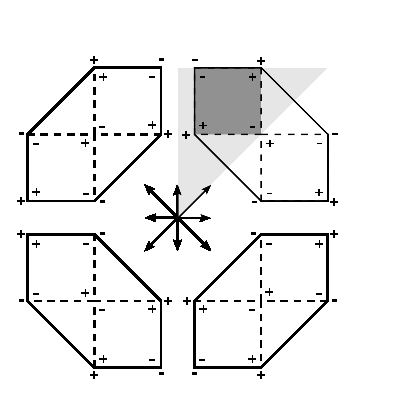
\includegraphics[width=0.95\linewidth]{drawing-1}
\caption{Splint $D_3= B_2\cup A_1+A_1$: the projection of the singular element $\Phi_{D_3}^{[1,1,2]}$ can be made from singular elements $\Phi_{A_1+A_1}^{[1,1]}$. Light-grey area is the fundamental Weyl chamber of subalgebra $B_2$.} 
\label{ris1} 
\end{minipage}
\hfill
\begin{minipage}[h]{0.47\linewidth}
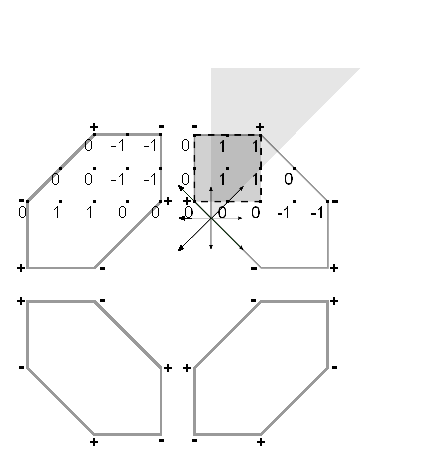
\includegraphics[width=0.9\linewidth,viewport=0 0 157 157,clip]{drawing-3}
\caption{The injection fan applied to the singular element $\Phi_{A_1+A_1}^{[1,1]}$ yields branching coefficients that are equal to 1.}
\label{ris2}
\end{minipage}
\end{center}
\end{figure}

A careful examination of the embedding $G_{2}\to B_{3}$ leads to exactly the same conclusion. 

So far we only considered special splints where both embedded systems are root systems. However, it
is possible to study the splints where it is not the case. Such splints obviously can not serve to
simplify calculation of the branching rules but one may use the properties of special embeddings and
the projections to creat a repesentation theory for the systems that are not root systems.

As the result we see that branching coefficients coincide with weight multiplicities for the splints
in the following table:
\begin{equation}
\label{tab:2}
\begin{array}{cc||c|c}
\hbox{type} & \hspace{0.25in}\Delta \hspace{0.25in} & \hspace{0.25in}\Delta
_{\frak{a}}\hspace{0.25in} & \hspace{0.25in}\Delta _{\sfr}\hspace{0.25in}
\\ \hline\hline
\hbox{(i)} & G_{2} & A_{2} & A_{2} \\
& F_{4} & D_{4} & D_{4} \\ 
\hbox{(*)} & B_{3} & G_{2} & A_{2}  \\
\hbox{(*)} & D_{r+1} & B_{r} & \oplus ^{r}A_{1}  \\
\hline
\hbox{(ii)} & B_{r}(r\geq 2) & D_{r} & \oplus ^{r}A_{1} \\
\hbox{(iii)} & A_{r}(r\geq 2) & A_{r-1}\oplus u\left( 1\right)  & \oplus
^{r}A_{1} \\
& B_{2} & A_{1}\oplus u\left( 1\right)  & A_{2}
\end{array}
\end{equation} 
here the splints marked with (*) are special splints.


\section{Conclusion}
\label{sec:conclusion}

The computation of branching coefficients is important for different physical models with a symmetry
breaking. This computation is drastically simplified if branching coefficients coincide with weight
multiplicities, since efficient Freudental formula can be used \cite{moody1982fast}. The classification
of splints for regular and special embeddings gives us all the cases when this coincidence takes
place. Aside from computational importance, this coincidence is very interesting from
representation-theoretic point of view, because it follows from the new unexpected connection between
different simple Lie algebras. 

There exist special embeddings of semisimple Lie algebras into simple Lie algebras. For such
embeddings the procedure of finding splints that allow to calculate branching coefficient is similar
to the one conducted above. While the results of the procedure are not presented in this paper they
can be obtained with little difficulty.

\section*{Acknowledgements}
\label{sec:acknowledgements}

We thank the organizers of the conference ``In Search of Fundamental Symmetries'' where some results
of this work were presented.

P.I. Kakin would like to acknowledge Saint Petersburg State University for the research grant
11.38.185.2014.


\bibliography{special-bibliography}{} 
\bibliographystyle{utphys}

\end{document}
